\chapter{Coherencia entre métrica transcripcional y espacio de conocimiento GO}
En los capítulos precedentes cuantificamos por medio de diversos índices la congruencia biológica de los grupos encontrados en el espacio de expresión génica. En este capítulo buscaremos cuantificar la coherencia entre los espacios de expresión génica y de conocimiento biológico desde una óptica diferente: desde la métrica en lugar de desde las agrupaciones.
\section{Alineamiento de núcleo-objetivo}
Una matriz de núcleo o matriz de Gram o matriz de kernel $K$ puede ser pensada informalmente como una matriz semidefinida positiva de similaridad de a pares entre puntos de un conjunto de datos. Para un conjunto de datos $\{x_1,...,x_m\}$ esta noción de similaridad esta dada en términos de una función $k$ llamada kernel tal que:
\begin{equation}
	K = K_{ij} = k(x_i, x_j)
\end{equation}
con $i,j=\{1,...,m\}$ y $k: \mathbb{R}^m \times \mathbb{R}^m \Rightarrow \mathbb{R}$. Una función $k(x, y)$ es un kernel si y solo si para cualquier conjunto finito de datos $C=\{x_1,...,x_m\}$ y para cualquier conjunto $\{a_1,...,a_m\} \in \mathbb{R}^m$ se tiene que:
\begin{equation}
	\sum_{i,j=1}^m a_ia_jk(x_i, x_j)\geq 0
\end{equation}
Se puede demostrar que esto implica que $K$ debe ser semidefinida positiva (SDP), es decir, $K=\sum_i \lambda _i v_i v_i'$, con $\lambda _i \geq 0$ los autovalores de la matriz $K$ y $v_i$ sus autovectores.\\
Intuitivamente, un kernel es una transformación que mapea pares de puntos en un espacio de alta dimensionalidad a un indice de similaridad entre los mismos mediante el uso de un producto interno.\\
Existen multiplicidad de kernels disponibles y para cada aplicación será necesario encontrar el adecuado.\\
Es de esperar que si es posible extraer información biológica del espacio de expresión genética, entonces dos puntos que son similares (en algún sentido a definir por el kernel elegido) en el espacio de expresión, también lo sean en el espacio GO (nuevamente, en algún sentido a definir por el kernel elegido). Para cada espacio habrá que definir un kernel adecuado.\\
Una forma de cuantificar la similaridad entre estos dos espacios es mediante una cantidad conocida como alineamiento núcleo-objetivo o KTA. El KTA de un kernel $k_1$ con respecto a un kernel $k_2$ del conjunto $C$ esta definido como:
\begin{equation}
	\hat{A}(S, k_1, k_2) = \frac{\langle K_1, K_2 \rangle _F}{\sqrt{\langle K_1, K_1 \rangle _F \langle K_2, K_2 \rangle _F}}
\end{equation}
Donde $\langle K_1, K_1 \rangle _F = \sum_{i,j=1}^m K1(x_i, x_j)K2(x_i, x_j)$ es el producto de interno de Frobenius entre matrices y $K_i$ son las matrices de kernels simétricas y semidefinida positivas de los espacios a comparar. Este índice tiene un rango entre $[0, 1]$.\cite{Cristianini2006}\\
Es posible extender este concepto a matrices simétricas indefinidas (no SDP) $S$ mediante diversas técnicas que consisten en transformar $S$ para obtener una $S'$ SDP. Esto es relevante para nosotros, porque matrices de similaridad basadas en similaridad semántica no suelen ser semidefinidas positiva. La que utilizaremos en este trabajo se conoce como \textit{corrimiento del espectro}. Si $S$ es simétrica entonces admite una descomposición en autovalores y autovectores tal que $S=U\Lambda U^T$ con $U$ una matriz ortogonal y $\Lambda$ una matriz diagonal de autovalores reales, es decir, $\Lambda = diag(\lambda _1,...,\lambda _m)$. Entonces, el corrimiento del espectro consiste en correr todo el espectro de $S$ por el mínimo necesario: 
\begin{equation}
	S_{corrida} = U(\Lambda + |\min{\lambda _{min}(S), 0}|I)U^T 
	\label{eq:matriz_corrida}
\end{equation}
Decidimos utilizar este método porque el mismo solo aumenta las autosimilaridades, sin modificar la similaridad entre dos puntos distintos, preservando la estructura de grupo al agrupar datos no necesariamente métricos.\cite{Chen22009}\\
Notar que esta medida es una medida global, ya que toma en cuenta todas las similaridades para calcular KTA.\\
\section{Espacio de expresión y GO}
Para cuantificar la coherencia métrica entre el espacio de expresión de cada tratamiento y las ontologías GOBPA, GOBPB y GOCC, utilizamos como kernel de espacio de expresión, $K_x$, la similaridad derivada de la correlación:
\begin{equation}
	k_x(g_i, g_j) = (\frac{correlacion(g_i, g_j)+1}{2})
	\label{eq:similaridad_de_correlacion}
\end{equation}
con $g_i$ y $g_j$ genes pertenecientes al tratamiento en cuestión.\\
Para el kernel del espacio de ontologías, utilizamos la similaridad definida en la ecuación \ref{eq:sim_rcmax} y transformamos la matriz en SDP por medio de \ref{eq:matriz_corrida}. La matriz se construyó tomando en cuenta todos los genes del tratamiento. Si un gen del tratamiento no se encontraba anotado en la ontología, se lo anotaba al nodo raíz y por lo tanto su similaridad con el resto de los genes era cero. Se calculó entonces para cada tratamiento y cada ontología, el KTA y se construyó además un control nulo de tipo 2, realizando 1000 reordenamientos aleatorios de las etiquetas de la matriz $K_x$.\\
Las figuras \ref{fig:kta_global_cc}, \ref{fig:kta_global_bpa} y \ref{fig:kta_global_bpb} presentan en un boxplot, para cada tratamiento y cada ontología, el KTA del control nulo, junto con un punto rojo para el KTA de expresión. 
\begin{center}
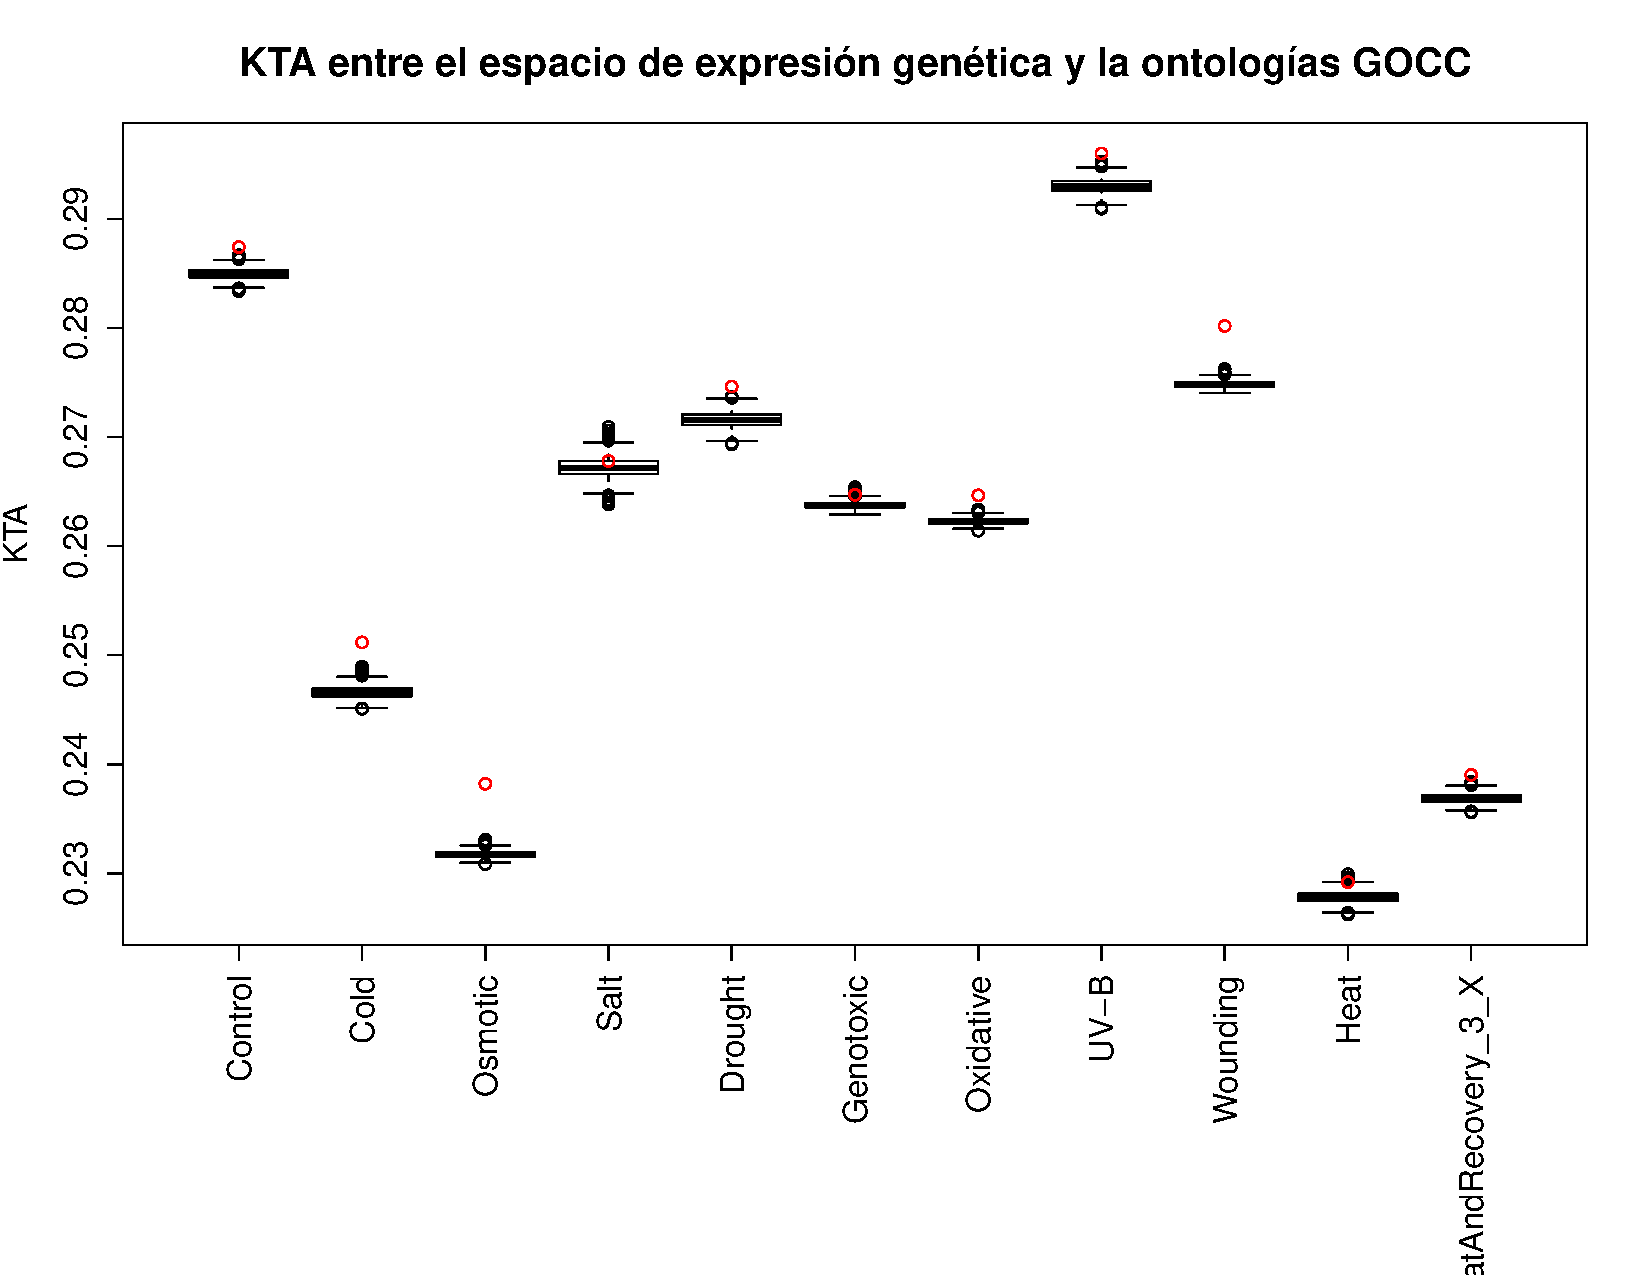
\includegraphics[height=0.4\textheight, width=0.7\textwidth]{kta_global_cc.pdf}
\captionof{figure}{KTA para distintos tratamientos entre espacio de expresión y ontología CC.}
\label{fig:kta_global_cc}
\end{center}
\begin{center}
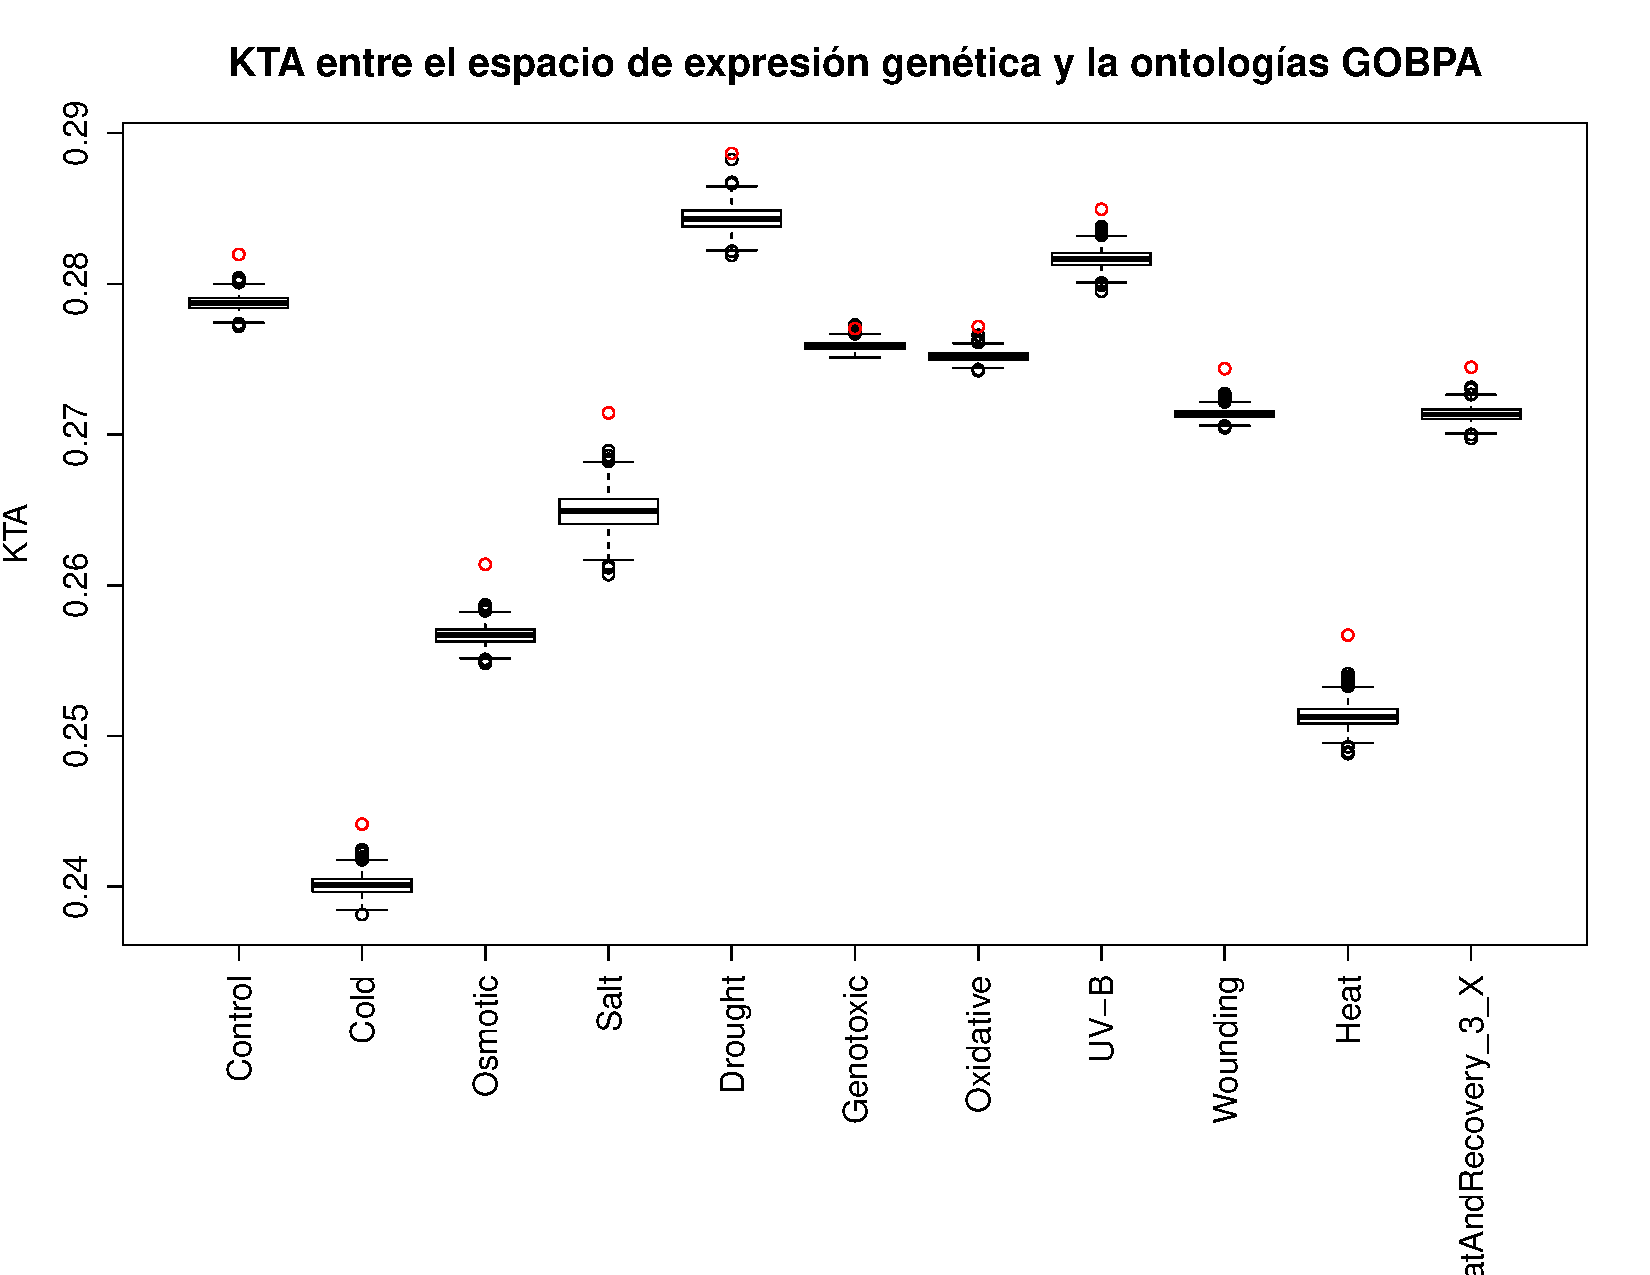
\includegraphics[height=0.4\textheight, width=0.7\textwidth]{kta_global_bpa.pdf}
\captionof{figure}{KTA para distintos tratamientos entre espacio de expresión y ontología BPA.}
\label{fig:kta_global_bpa}
\end{center}
\begin{center}
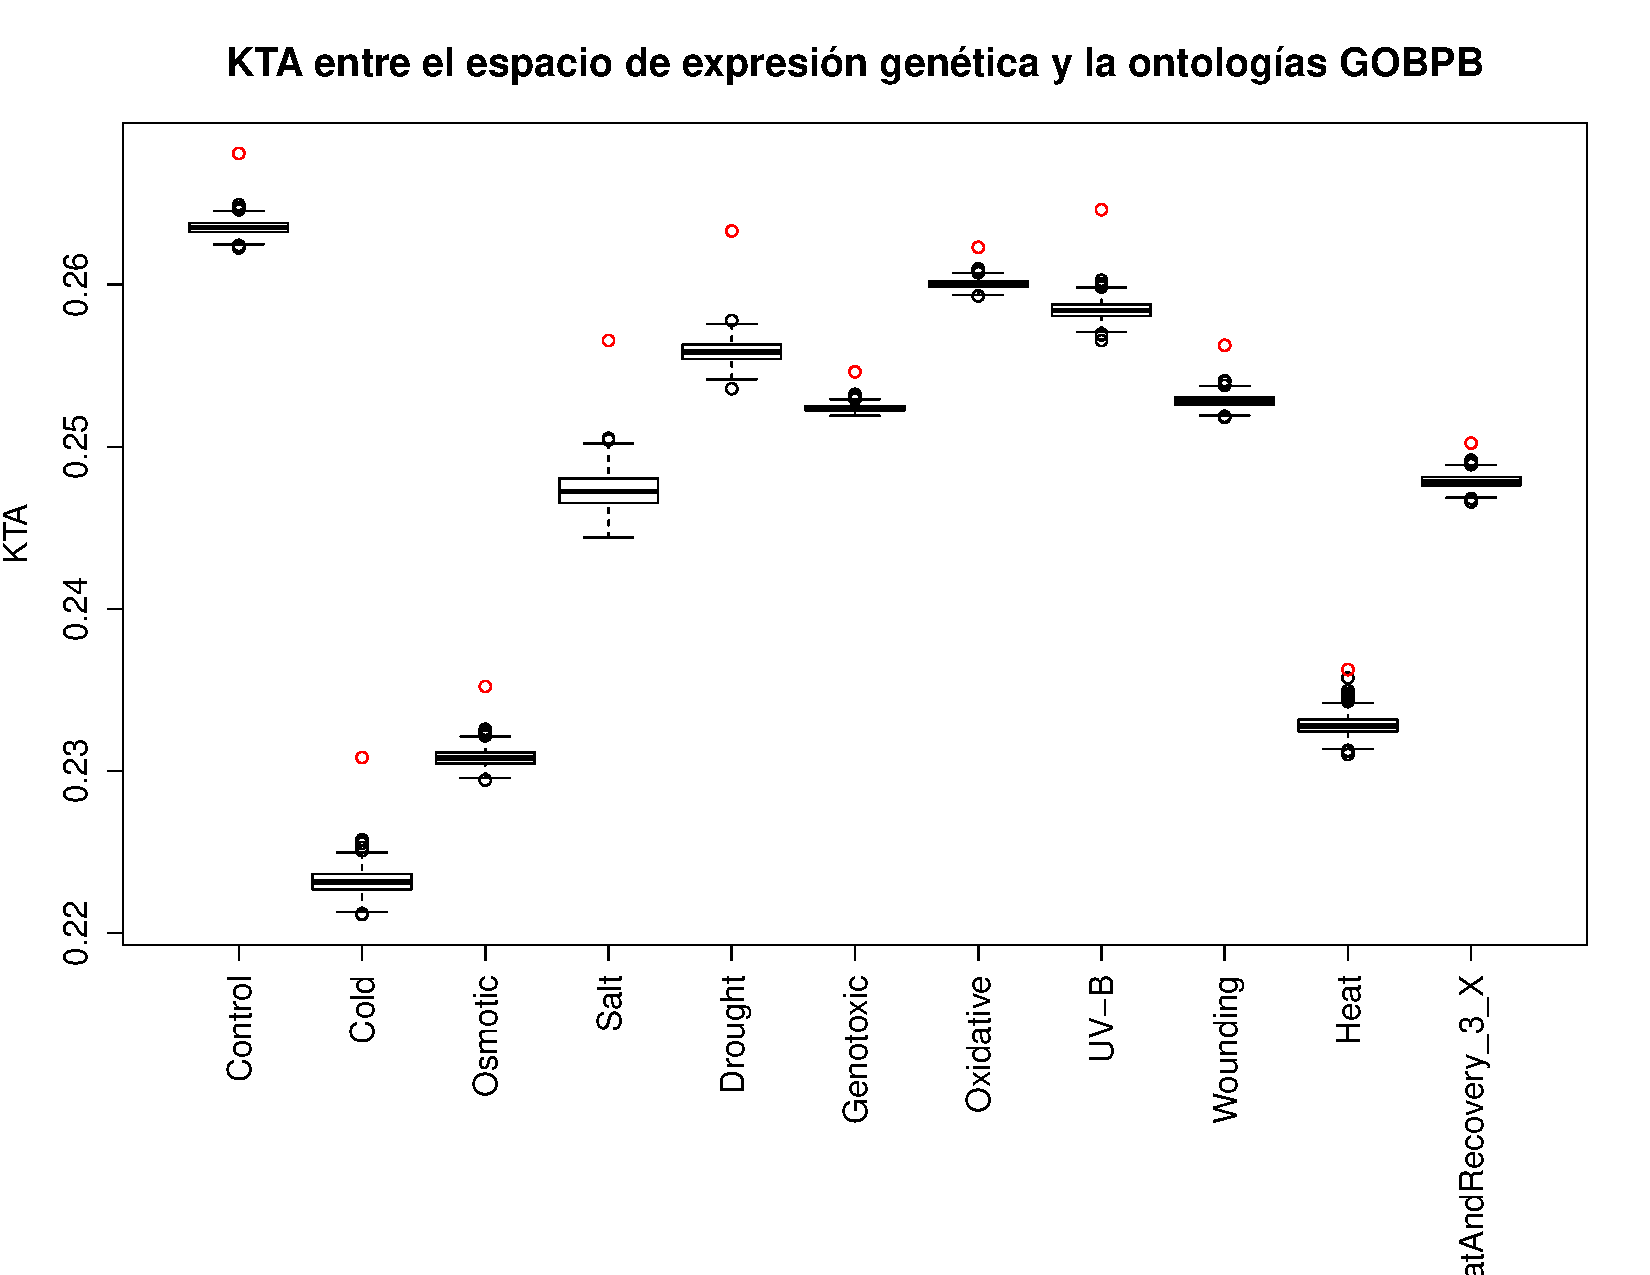
\includegraphics[height=0.4\textheight, width=0.7\textwidth]{kta_global_bpb.pdf}
\captionof{figure}{KTA para distintos tratamientos entre espacio de expresión y ontología BPB.}
\label{fig:kta_global_bpb}
\end{center}
En todos los casos encontramos que el KTA de expresión supera todos los valores del KTA de control nulo, lo que soporta la idea de que existe un grado de coherencia no trivial, de orden global, entre la métrica de expresión transcripcional y la métrica del espacio de conocimiento biológico, inferido a partir de la estructura de GO.
\section{Alineamiento de núcleo-objetivo local}
En la sección anterior presentamos una forma de cuantificar globalmente la coherencia entre la métrica transcripcional y el espacio GO mediante el índice KTA. Es posible redefinir este índice para obtener una medida de alineamiento de estos dos espacios pero de forma local, en vecindades transcripcionales. La idea de esta nueva medida apunta a cuantificar e identificar regiones acotadas del espacio transcripcional (i.e. grupos de genes) donde exista un alineamiento espacio-transcripcional vs. espacio-GO diferente a la media. Este índice nos será de gran utilidad en un análisis posterior para caracterizar la congruencia biológica en grupos de genes de similar comportamiento transcripcional y para definir una métrica mixta, que permita definir agrupamientos de genes que presente alto grado de coherencia no solo a nivel transcripcional, sino también en el espacio de conocimiento biológico.\\
Para definir vecindades transcripcionales consideramos redes de k-primeros-vecinos-mutuos, donde cada nodo es un gen y cada arista tiene un peso $w_{ij}$ entre $[0, 1]$ dado por la similaridad de correlación entre los dos genes $g_i$ y $g_j$ que son unidos por esa arista. Construimos una red $k=30$, que llamamos $30kmnn$, y estudiamos su topología \footnote{Exploramos diferentes alternativas en este punto que incluye el uso de redes de k primeros vecinos en lugar de k primeros vecinos mutuos, y de un número variable de primeros vecinos. Encontramos que la red $30kmnn$ presentada en el trabajo era un buen compromiso entre cobertura y tiempo de computo.}.\\
\subsection{Vecindades transcripcionales}
Como primer paso para entender alguna de las particularidades y limitaciones de nuestra caracterización de las vecindades transcripcionales estudiaremos a la red $30kmnn$ mediante dos observables topológicos, la distribución de grado y la intermediación central o \textit{betweenness centrality}.\\
Además, compararemos la red con dos modelos de redes aleatorias, el modelo de Erdös Renyi, que consiste en construir una red aleatoria con $N$ nodos, conectando pares elegidos al azar y omitiendo múltiples conexiones entre dos mismos nodos hasta alcanzar una cantidad total de $K$ aristas impuestas a priori \cite{Erdos1959}, y el modelo configuracional, que genera una red aleatoria a partir de un recableado de conexiones que mantiene fijo el grado de cada nodo, es decir, no altera la distribución de grado $P(k)$ de la red original \cite{Molloy1995}.
\subsection*{Distribución de grado}
El grado $k_i$ de un nodo de la red es la cantidad de primeros vecinos que tiene el nodo.\\
La distribución de grado $P(k)$ es entonces la probabilidad de un que nodo $i$ tomado al azar tenga grado $k$.\\La figura \ref{fig:erdos_renyi_vs_30kmnn} muestra la distribución de grado en escala logarítmica de la red de 30 primeros vecinos mutuos y un modelo nulo de Erdös-Rényi con la misma cantidad de nodos y aristas para el tratamiento frió (1951 nodos y 18436 aristas). Se observa que el grado máximo que alcanzan estas distribuciones está relacionado directamente con el $k$ utilizado, ya que a lo sumo un nodo tendrá $k$ primeros vecinos ($k$ aristas). El hecho de tener un gran número de nodos con k máximo sugiere que ya alcanzamos la ``saturación'' en una representación basada en interacciones de vecinos mutuos. Vemos de la figura que la distribución obtenida se aleja de la Poissoniana correspondiente al modelo nulo Erdös-Rényi.
\subsection*{Intermediación central o betweenness centrality}
La longitud de un camino entre dos nodos se define como la cantidad de aristas que se recorren para llegar de un nodo al otro. El camino (o caminos) más corto es aquél camino cuya longitud es la menor entre todos los caminos. La longitud de un camino más corto se conoce como distancia geodésica.\\
El betweenness centrality de un nodo $i$ es igual a la cantidad de caminos más cortos desde todos los nodos a todos los otros nodos que pasan por el nodo $i$. Es una medida de la influencia del nodo $i$ en la red, ya que un nodo con alto betweenness centrality recibirá una gran parte de la carga de la red, suponiendo que la carga se distribuye a través de los caminos más cortos.\\
Muchas redes reales presentan algunos nodos de alta conectividad, llamados conectores o \textit{hubs}, por donde pasa la mayor parte de la carga de la red.\\
La figura \ref{fig:betweenness_er_30_conf} presenta en escala logarítmica la relación entre el betweenness y el grado $k$ de los nodos de la red $30kmnn$ obtenida para el tratamiento ``Frío'' (1951 nodos, 18436 aristas). En círculos grises, la de Erdös-Rényi, en triángulos amarillos y la configuracional, en rombos rojos.\\
\begin{figure}[H]
    \centering
    \begin{subfigure}[t]{0.45\textwidth}
    \centering
    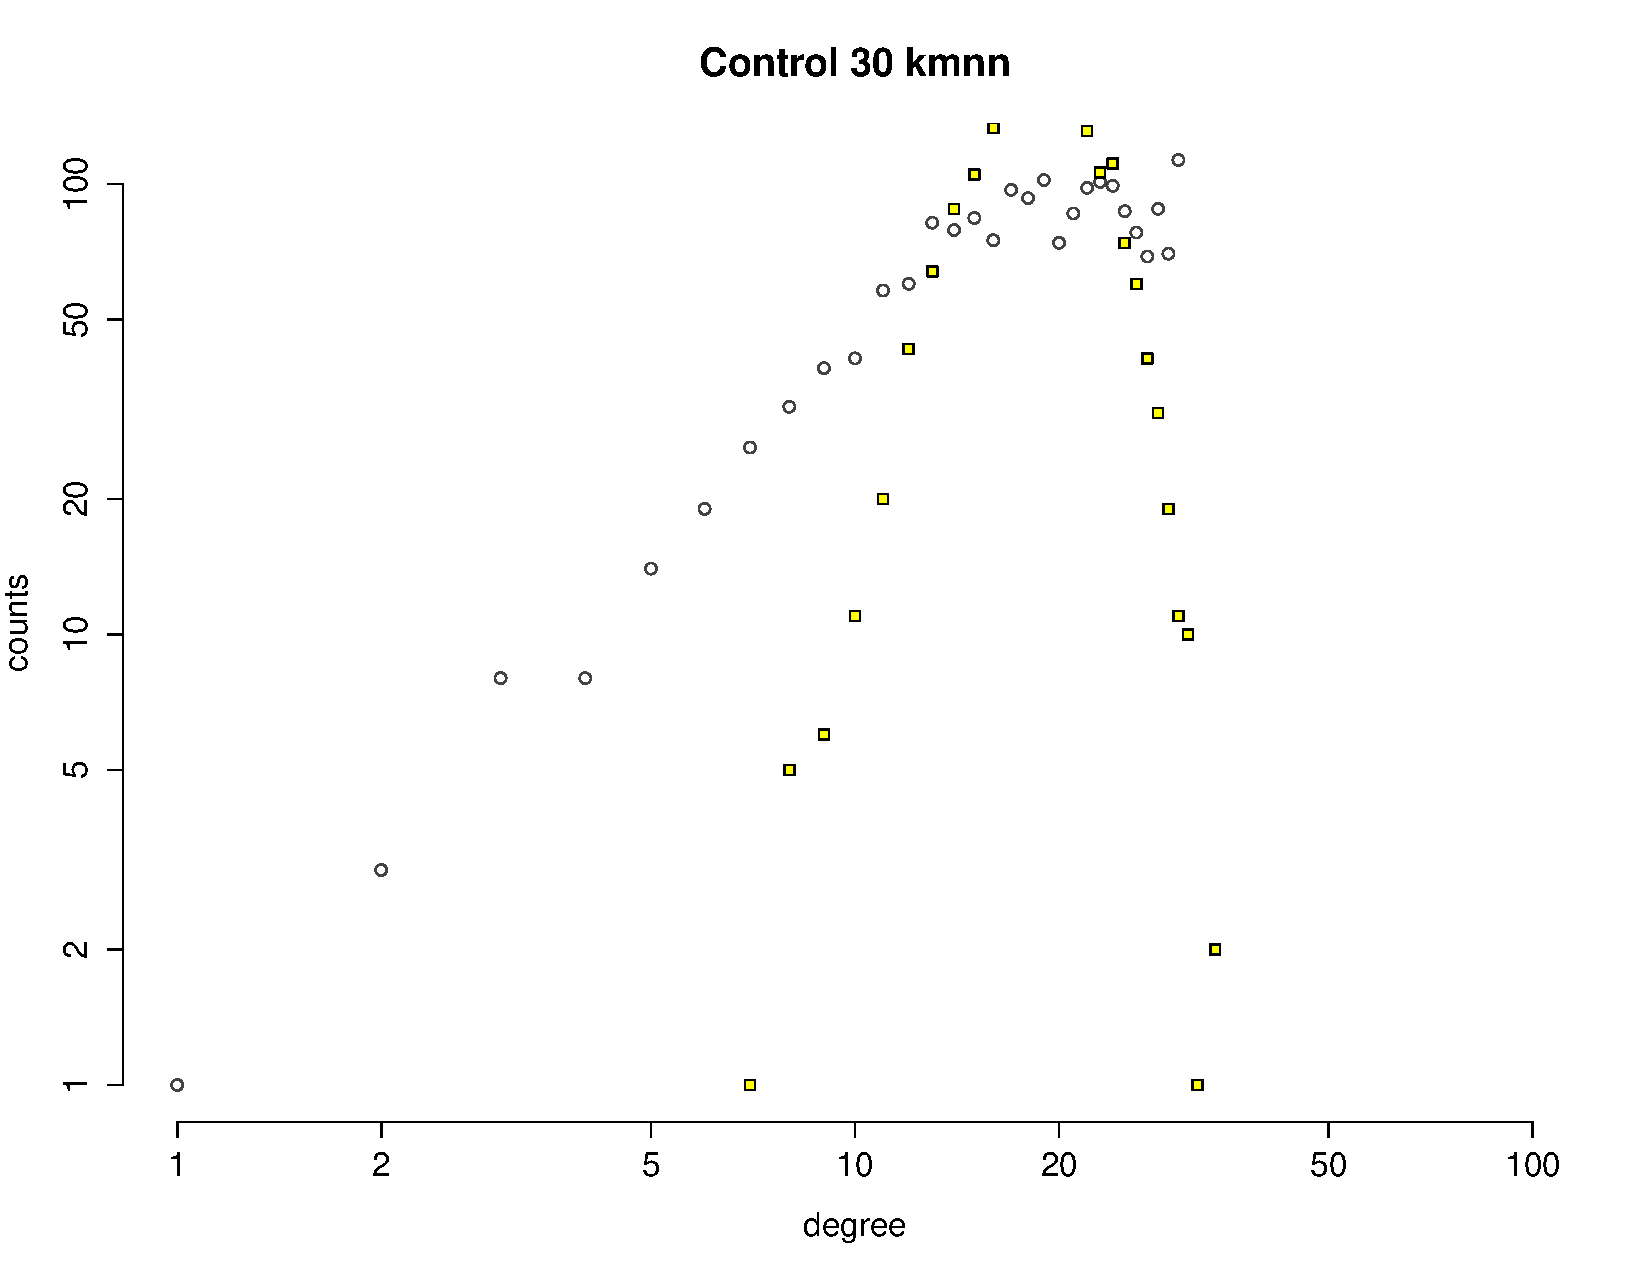
\includegraphics[width=1\textwidth]{erdos_renyi_vs_30kmnn.pdf}
    \caption{Distribución de grado para los nodos de la red $30kmnn$ para el tratamiento 'Frío' (círculos vacíos) y para una red de Erdös-Rény (cuadrados amarillos) con idéntica cantidad de nodos y aristas.}
    \label{fig:erdos_renyi_vs_30kmnn}
    \end{subfigure}    
    \centering
    \begin{subfigure}[t]{0.45\textwidth}
    \centering
    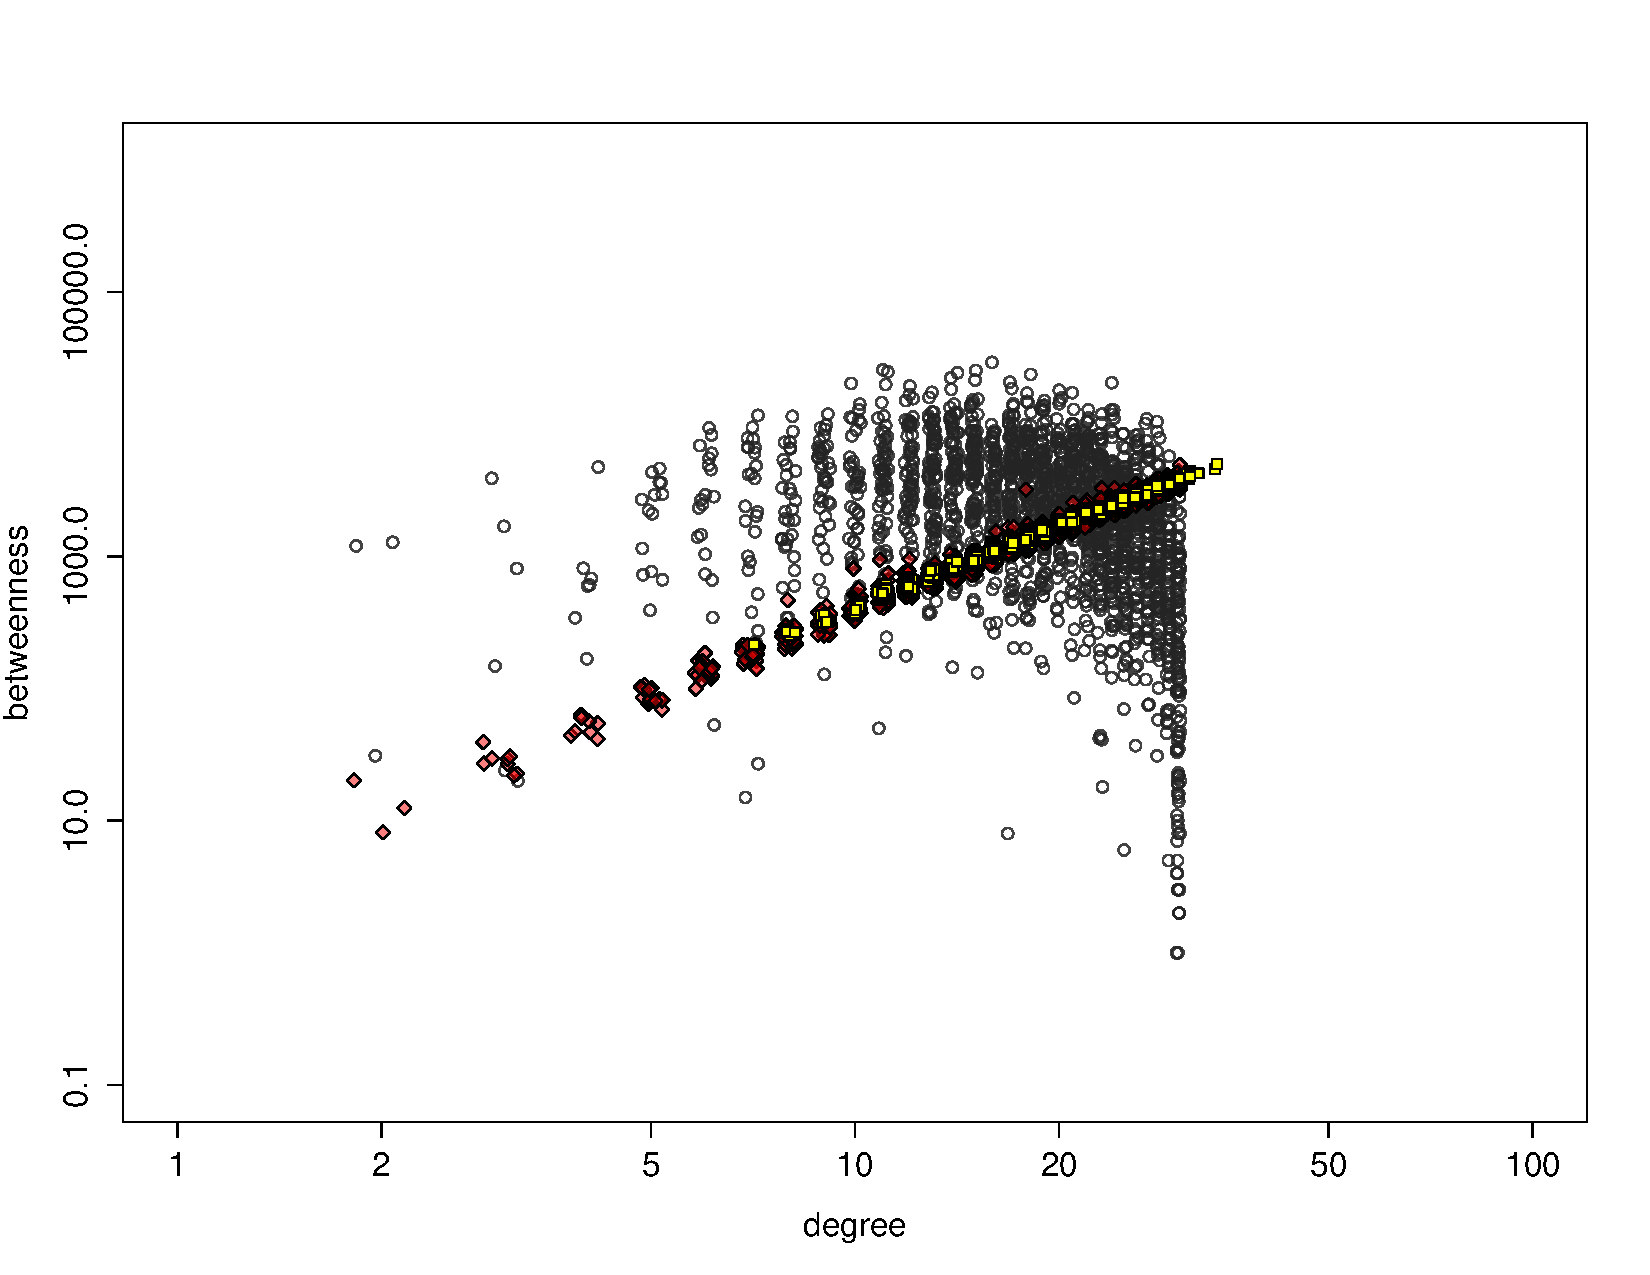
\includegraphics[width=1\textwidth]{betweenness_er_30_conf.pdf}
    \caption{Distribución de betweenness centrality en función del grado de la red para los nodos de las redes $30kmnn$ para el tratamiento 'Frío', Erdös-Rényi y configuracional.}
    \label{fig:betweenness_er_30_conf}
    \end{subfigure}        
    \caption{Distribución de grado y de betweenness centrality para los nodos de la red $30kmnn$ y modelos nulos}
\end{figure}
En todos los casos se observa una correlación positiva entre el betweenness y el grado de la red, pero cabe destacar que para un grado fijo $k$, la red $30kmnn$ presenta una mayor dispersión en el betweenness que las otras. Existen en la red $30kmnn$ nodos de grados intermedios con altos valores de betweenness, a la vez que hubs con bajísimos valores de betweenness. Esto es compatible, por ejemplo, con la existencia dentro de la red de módulos, con hubs locales, interconectados entre si mediante nodos de grado medio-bajo. En todo caso, estos resultados sugieren la existencia de estructura y patrones de conectividad no triviales en la red $30kmnn$.
\subsection{KTA local red 30kmnn}
La red $30kmnn$ tiene embebida en su estructura de inteconectividades la información sobre los entornos locales de cada gen. Para obtener una caracterización del grado de coherencia local entre espacios transcripcionales y GO, para cada arista de la red $30kmnn$ de cada tratamiento, encontramos su vecindario local a primeros vecinos (los $n_x$ primeros vecinos de los nodos unidos por la arista) y construimos la matriz de similaridad de correlación reducida, consistente en la similaridad de correlación entre esos nodos y sus primeros vecinos. Generamos además la matriz de similaridad semántica reducida usando únicamente los genes anteriores, para cada una de las ontologías GOBPA, GOBPB y GOCC (aquellos genes que no estaban anotados en las ontologías, fueron anotados en la raíz de cada una respectivamente).\\
Observamos que la cantidad de nodos vecinos anotados en la ontología, $ny$, depende linealmente de la cantidad de nodos vecinos en la red, $nx$, como muestra la figura \ref{fig:nx_vs_ny}. Por otro lado, podemos ver que el promedio de los pesos en una vecindad de una arista anotados en la ontología, $wynanotados$, presenta una gran dispersión en su relación con los pesos de las aristas, como se observa en la figura \ref{fig:wy_vs_wynanotados}. Esto implica que el comportamiento en una vecindad no puede ser predicho a partir del conocimiento de un edge, sino que es necesario tomar toda la vecindad en su conjunto.
\begin{sidewaysfigure}[t!]
    \centering
    \begin{subfigure}[t]{0.45\textwidth}
    \centering
    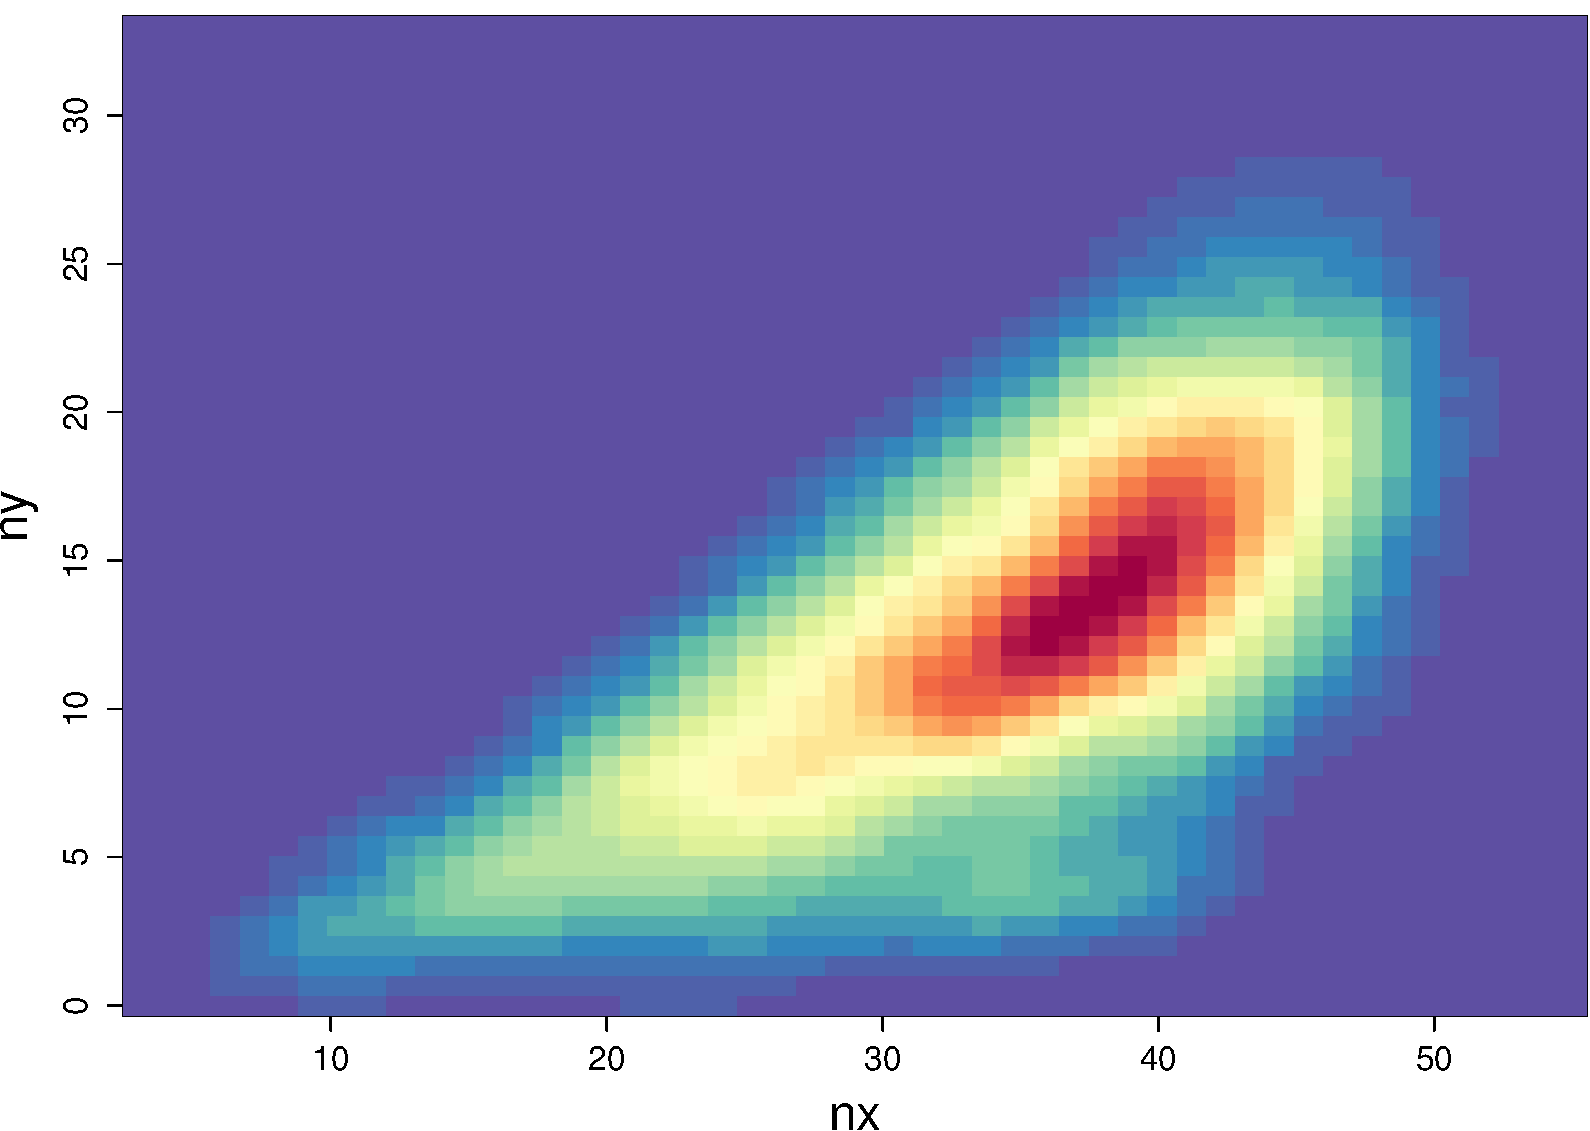
\includegraphics[width=1\textwidth]{nx_vs_ny.pdf}
    \caption{Primeros vecinos en GO en función de primeros vecinos en expresión.}
    \label{fig:nx_vs_ny}
    \end{subfigure}    
    \begin{subfigure}[t]{0.45\textwidth}
    \centering
    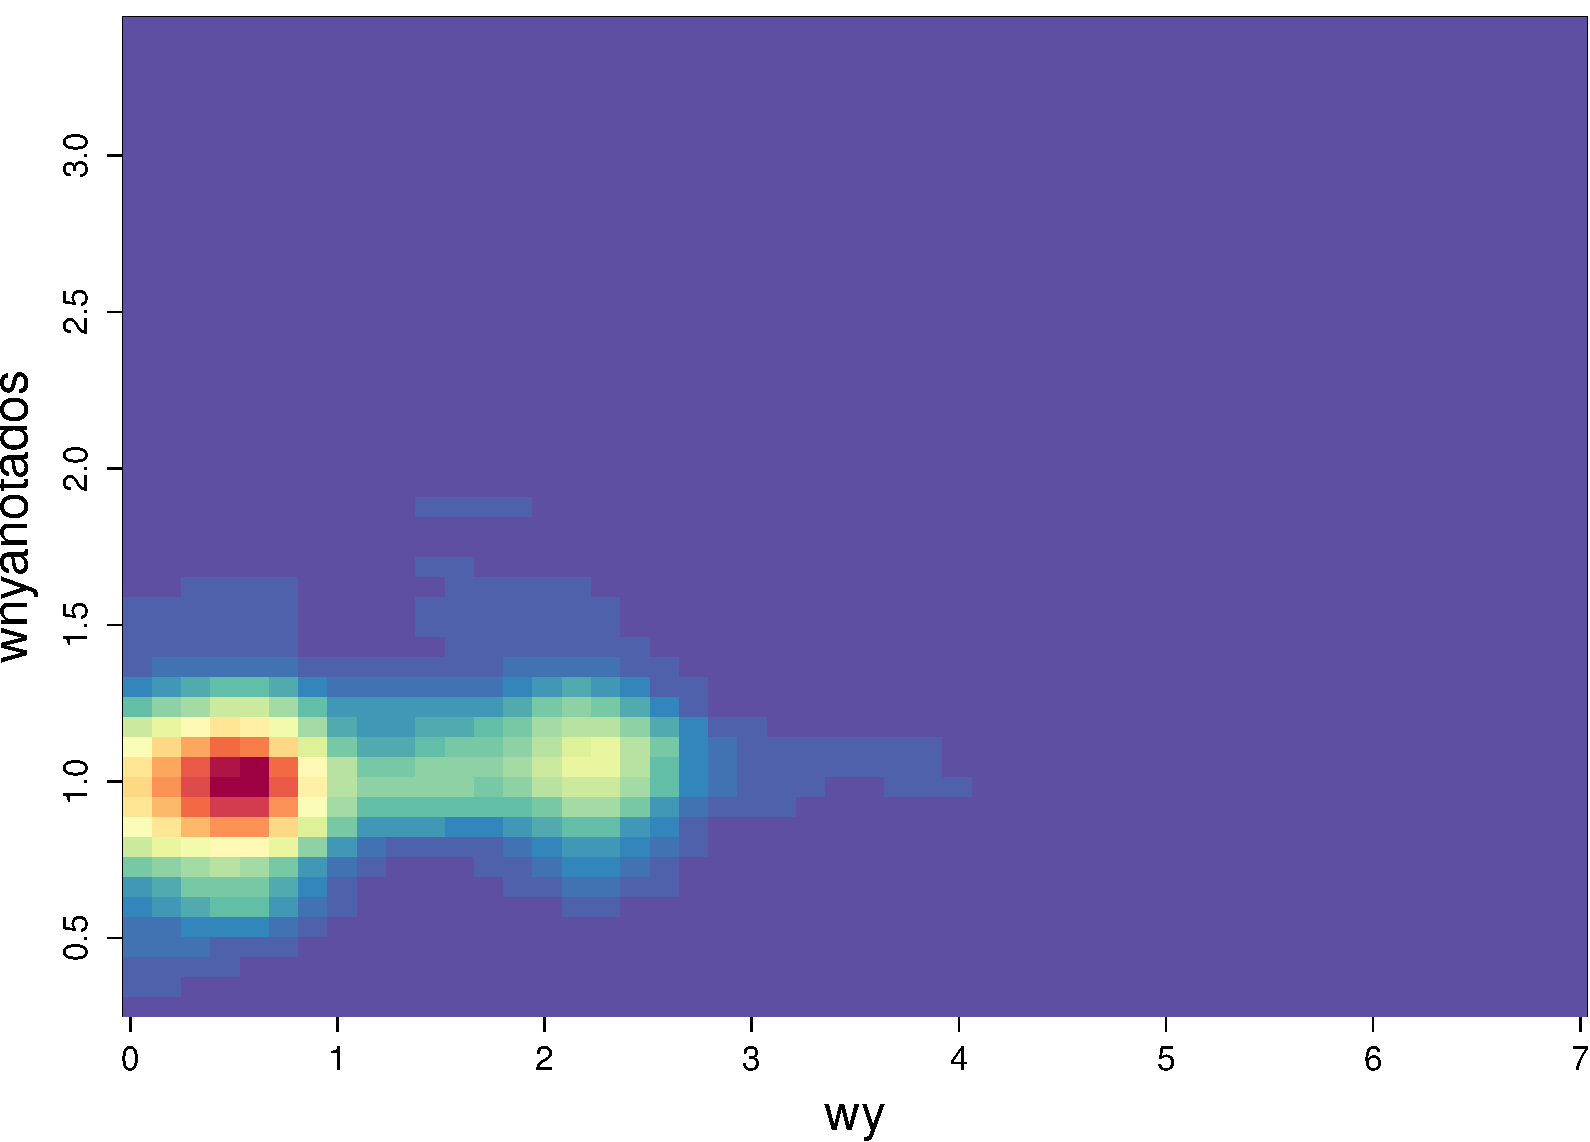
\includegraphics[width=1\textwidth]{wy_vs_wynanotados.pdf}
    \caption{Promedio de pesos anotados en GO en función de pesos de las aristas.}
    \label{fig:wy_vs_wynanotados}
    \end{subfigure}    
    \begin{subfigure}[t]{0.45\textwidth}
    \centering
    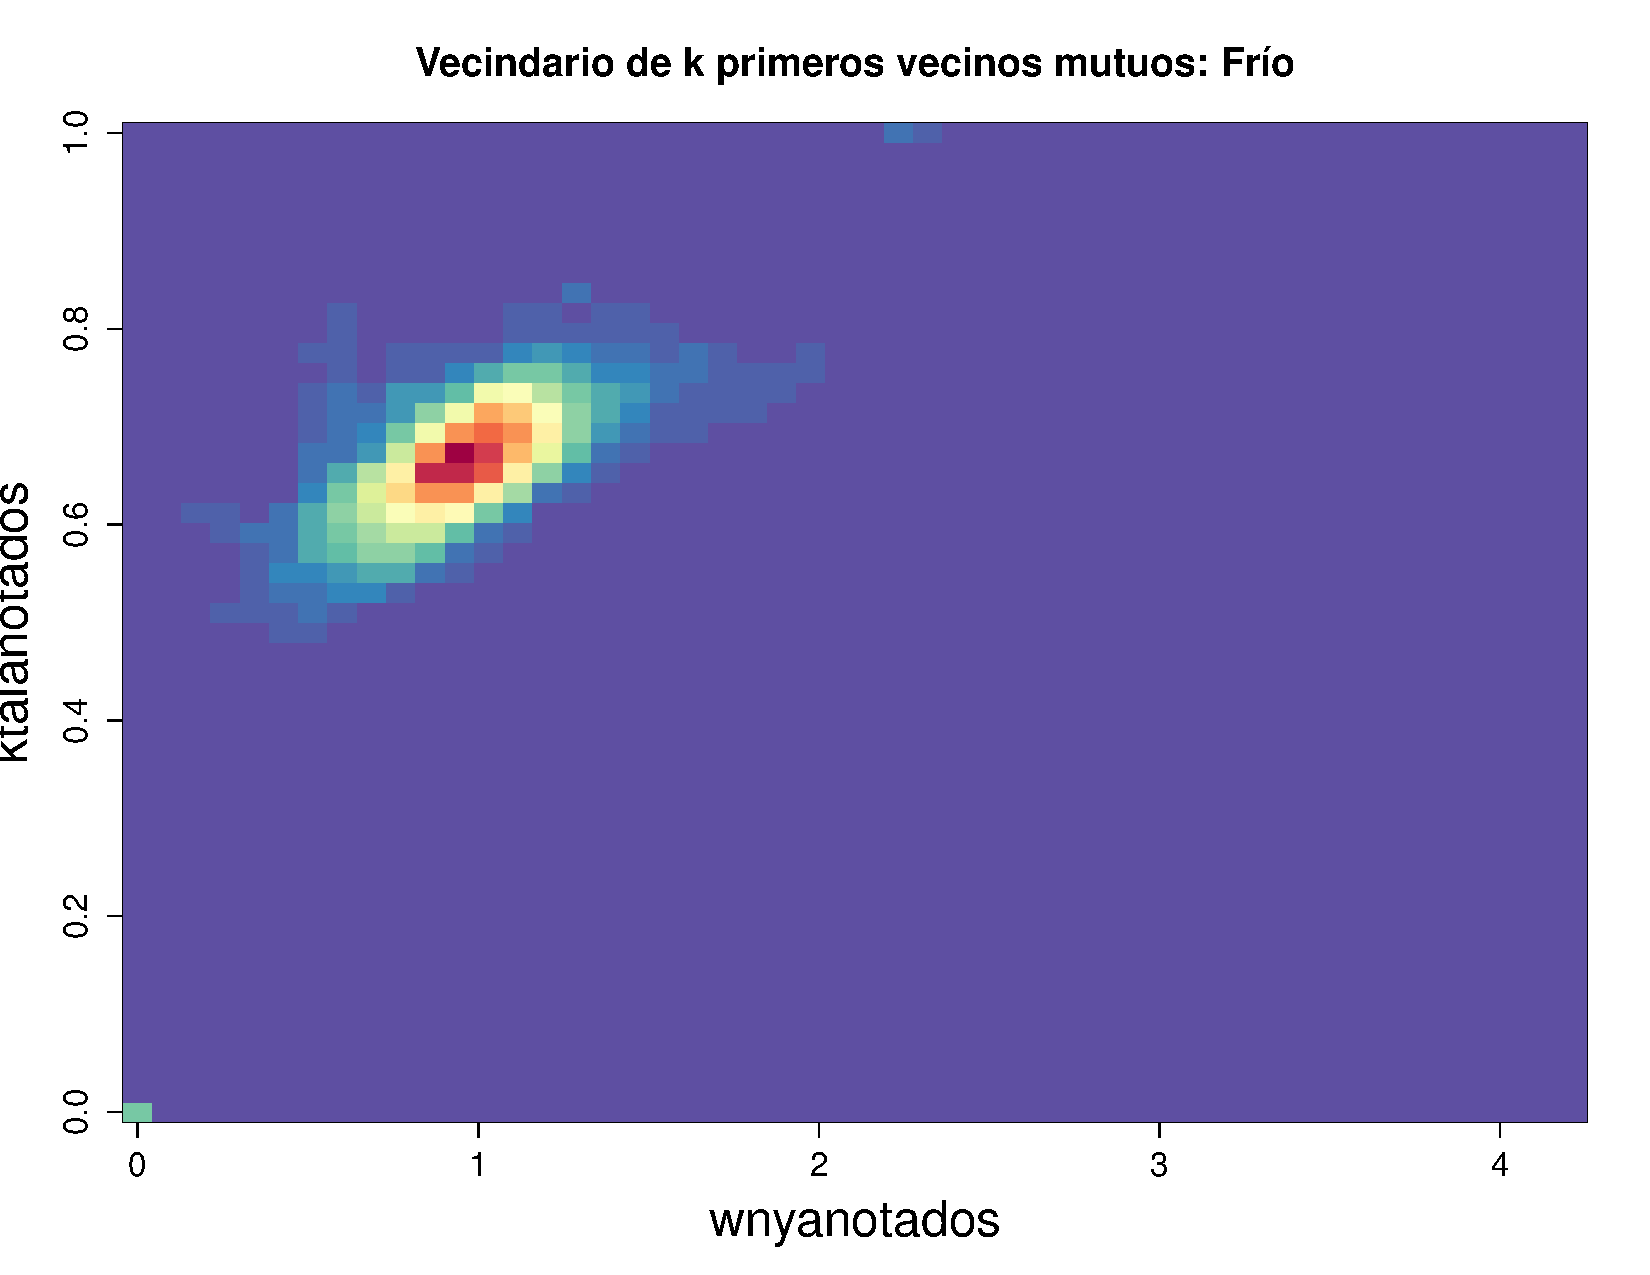
\includegraphics[width=1\textwidth]{lktaanotados_vs_wnyanotados.pdf}
    \caption{KTA local de los anotados en función del promedio de pesos anotados en GO.}
    \label{fig:lktaanotados_vs_wnyanotados}
    \end{subfigure}    
    \begin{subfigure}[t]{0.45\textwidth}
    \centering
    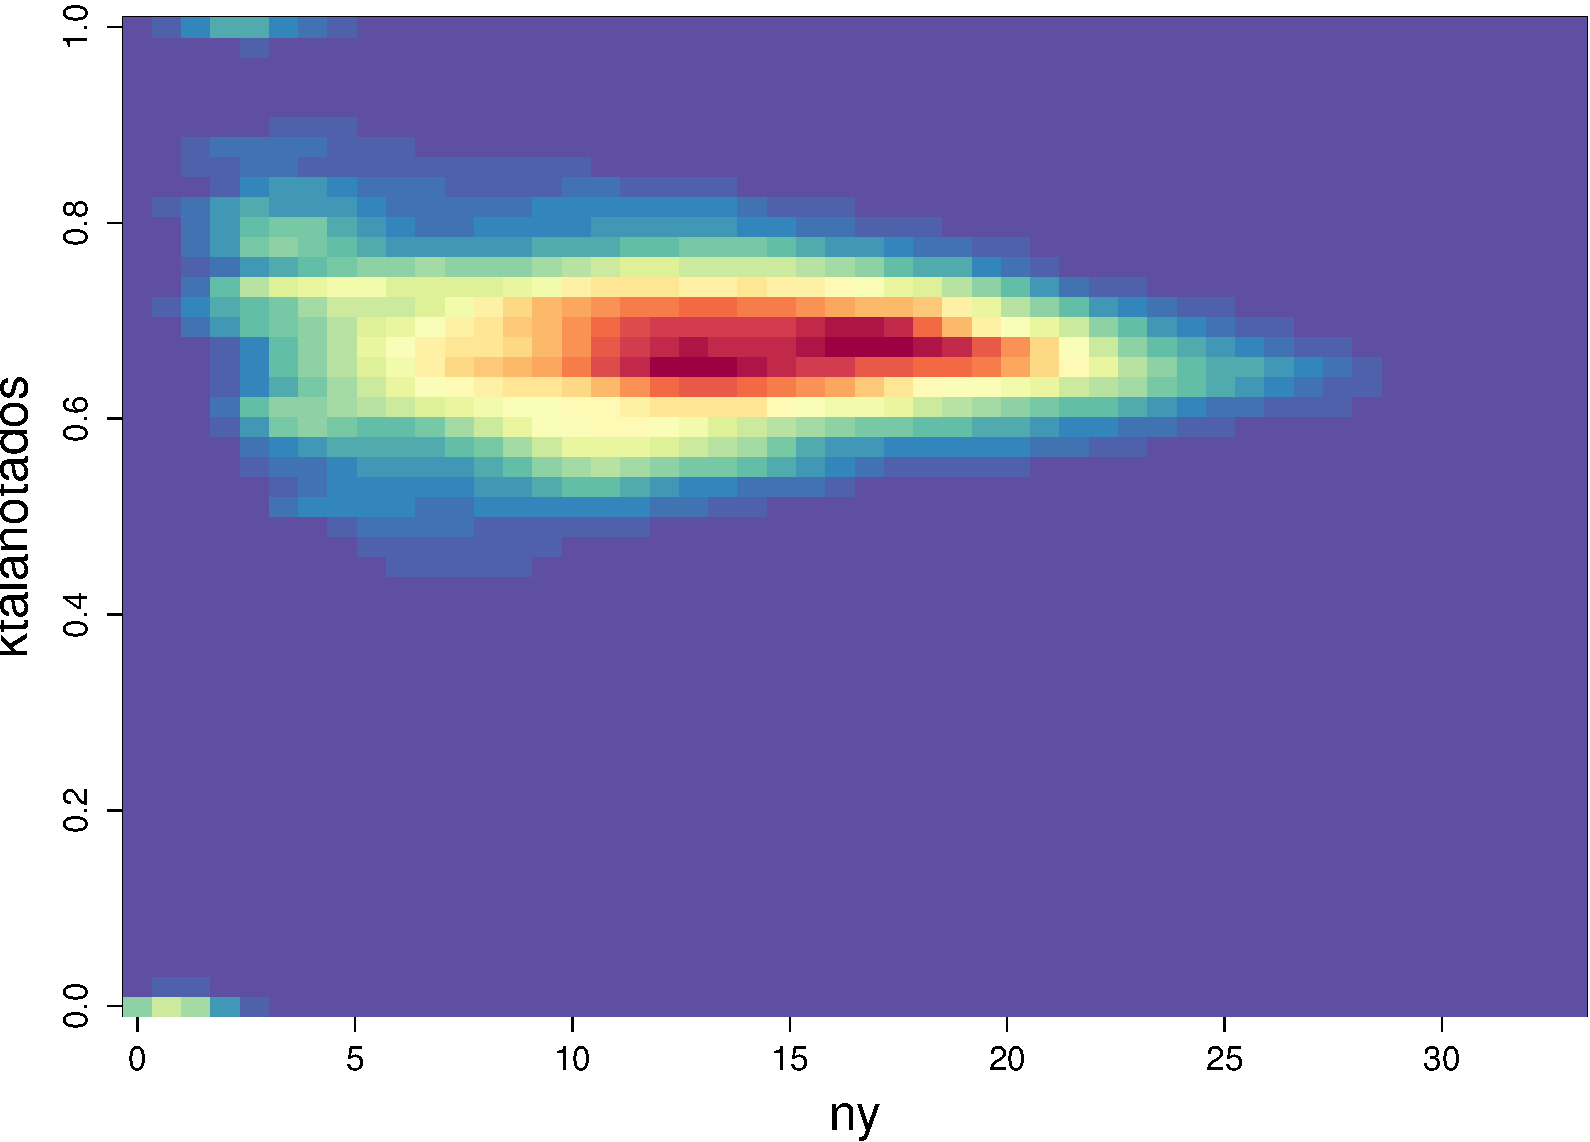
\includegraphics[width=1\textwidth]{lktaanotados_vs_nyanotados.pdf}
    \caption{KTA local de los anotados en función de la cantidad de vecinos anotados en GO.}
    \label{fig:lktaanotados_vs_nyanotados}
    \end{subfigure}            
    \label{fig:ktalocal}
    \caption{Caracterización de KTA local para tratamiento 'Frío'.}
\end{sidewaysfigure}
A partir de estas relaciones, introduciremos el índice KTA local como el índice KTA aplicado a las matrices reducidas de ambos espacios, previamente transformadas en SDP. Para caracterizar su comportamiento nos interesa observar primero que el comportamiento de este índice depende linealmente de $wynanotados$, como muestra la figura \ref{fig:lktaanotados_vs_wnyanotados}, siendo entonces coherente con el promedio de las aristas de su vecindad, lo que da cuenta que la información contenida en la ontología GO está relacionada con el índice KTA local. Por otro lado, de la figura \ref{fig:lktaanotados_vs_nyanotados} podemos verificar que no existe una dependencia fierte del KTA local con la cantidad de vecinos anotados $nyanotados$. Por lo tanto, el KTA local presenta valores más altos para vecinos con alta coherencia biológica, independientemente de la cantidad de vecinos que se tome en cuenta.
